\chapter{Test procedure}
\label{results}
After developing a translation concept, it is time to use it in practice.
In this chapter we will discuss how to develop the deadlock property we want to check and the results of our verification run.
Furthermore, we examine the used net representations and the test programs that were used in the development process.

\section{Petri-Net Representation}
\label{app_petri}
Implementing a basic graph structure to represent our Petri-Net is not very difficult.
But to be compatible with a Model checker we have to use some interface or a standard that
defines a commonly known structure.
Luckily there exists an XML-based standard for Petri-Nets called \textbf{Petri Net Markup Language}\cite{pnml}\cite{kindler2006petri} or \textbf{PNML}.
However, LoLA -- the model checker that we actually used -- defines it own representation.
And a third representation that comes in handy for visualization and debugging is \textbf{DOT}\cite{koutsofios1996drawing}, a simple language for graph definitions.
All languages are comparable in their core idea.
They all list nodes (places, transitions) and arcs of the graph. 
Additionally, the Petri-Net representations encode information for token count and arc weight.
Since all the three representation serve their own purpose, they were all integrated as target representation in our prototype.

\section{Model Checking}
\label{app_mc}
To test and inspect our results we have the choice between different tools.
An inspiration of performant tools like TAPAAL\cite{tapaal}, ITS-tools\cite{its-tools} or LoLA\cite{lola}\cite{schmidt2000lola} can be found in the results of the `Model Checking Contest'\cite{mcc}.
However, for a proof of concept it is not very important which model checker is used, since we will verify small test programs;
Performance is not the biggest concern at this time.
This is why LoLA was chosen by personal preference for this work.

Having a model checker and a Rust program that is translated to a Petri-Net, the last thing we need is a property to check for.
We want to search for deadlocks in the source program.
That means that the program execution is blocked unexpectedly and no operation can be executed.
This translates nicely to a dead Petri-Net where no transition is enabled and the net reached a final state.
We have to be careful though: there are states where the Petri-Net is expectedly dead;
Program termination is by definition a state there execution stops.
This means that if we reach either the \textit{program end} or the \textit{panic end} place, our net is expected to be dead.
To check for an unexpected deadlock we need to make sure that our termination places are not marked: $program\_end = 0\ \&\ panic = 0$.
Additionally, the net has to be dead.
In LoLA this is expressed with the keyword $DEADLOCK$.
So the state we want to discover would be $\Phi=DEADLOCK\ \& (program\_end = 0\ \&\ panic = 0)$.
The final part we have to consider is the temporal aspect.
To specify that our state property holds eventually and to find an applicable path, we can use the operators $EF\varphi$ in combination.
Its semantic is that the given property is satisfied in any of the successive paths at some point (or state).
So our final formula would look like this:
$$\Phi = EF(DEADLOCK\ \& (program\_end = 0\ \&\  panic = 0))$$

\section{Test Programs}
\label{app_test}
If we want to get some confidence in our translation process we have to see if it behaves as expected.
Initially, the basic functionality should be tested against the simplest programs to fail early.
And what could be simpler than the empty program from listing \ref{empty-program}?
Beside giving a good starting point for a testable implementation, the fact that all terminating programs have a deadlock should also get obvious here at the latest!

Other programs that can strengthen the confidence in the translation process include some important language features, like our simple function call from listing \ref{function_call_program} or an endless program (which actually is completely deadlock free):
\lstset{language=Rust,caption={An endless program},label=endless-program, frame=none, stepnumber=5, backgroundcolor=\color{verylightgray}}

\begin{lstlisting}
pub fn main() -> ! {
    loop {}
}
\end{lstlisting}
However, non of these programs are significant for what we really want to achieve: deadlock detection.
For this, we use our very first example program from listing \ref{deadlock_program}.
If our Petri-Net model is worth something the model checker should detect a deadlock for this program and none if we remove the last line (lock the mutex only once).

\section{Translation target}
\begin{figure}
  \centering
  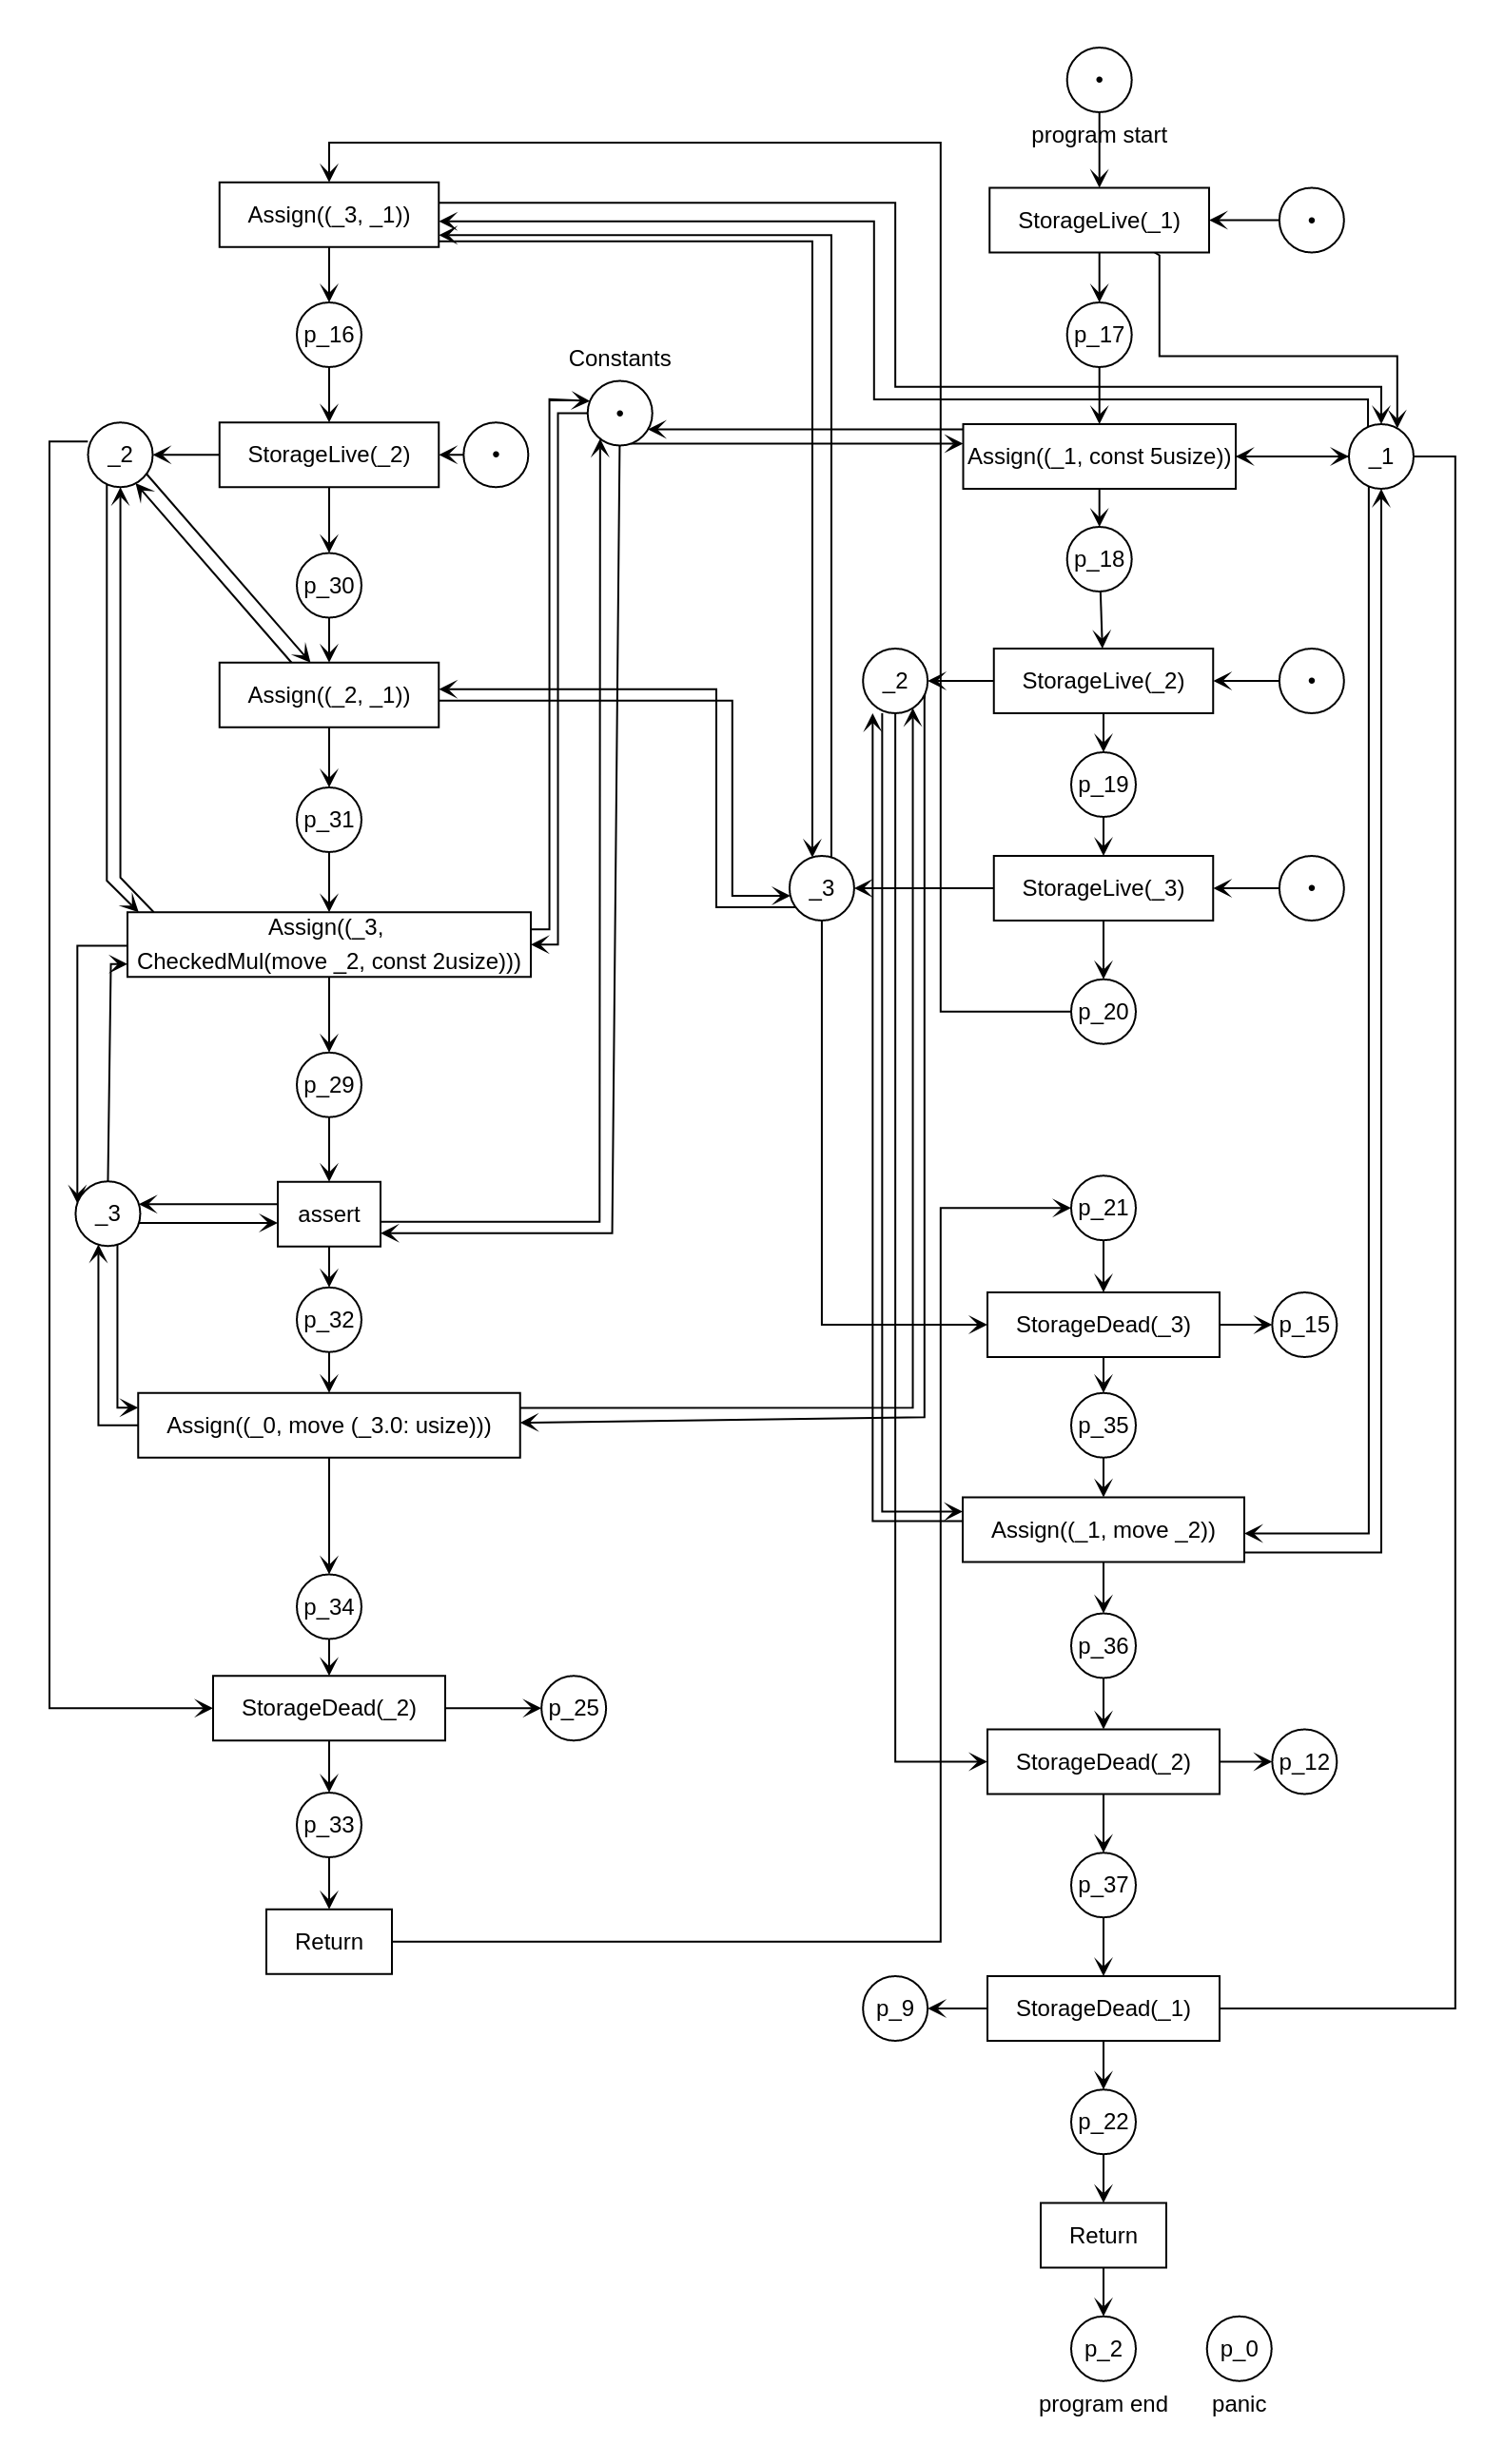
\includegraphics[width=0.9\textwidth]{../diagrams/FunctionCallNet.png}
  \caption{Translated Petri-Net}
  \label{function_call_net}
\end{figure}
In figure \ref{function_call_net} we can see the generated net for the function call program from listing \ref{function_call_program} (since this is small enough to show and big enough to not be trivial).
This is the true data that was produced for the dot target, so we cannot immediately see the virtual boundaries for statements basic blocks and functions.
To make the structure more clear the nodes where rearranged so that the called function is on the left and the main function on the right.
The initialized places of the locals where renamed to show their MIR name (locals are scoped by functions so their names are not unique).

We can see a path from program start to program end;
The panic place is unconnected because the program cannot panic.
Local life cycles are also visible as a single edged path from marked uninitialized place to unmarked dead places.
In contrast, variable manipulation always has parallel incoming and outgoing edges.
On a closer look we can see that local $\_3$ of the called function has no storage live or storage dead statements.
This is actually a correct representation of the MIR graph:
for some reason the storage statements are not generated for some lvalues (in this case the lvalue from checked multiplications).
If this is expected behavior is not known at the time of writing;
A bug report\footnote{https://github.com/rust-lang/rust/issues/67400} has yet to be solved.
Unfortunately this behavior introduces an unintended deadlock into our translation since depending transitions can only fire if the initialized places where previously marked.
To use the net for verification we have to work around this issue until it is fixed (or until the cause is modeled correctly).
To be able to continue testing, simply all \textit{initialized} places where marked as well.
This way the involved transitions can fire, but only if the previous statement produced a token on the connecting place (the program counter place).
But now, an additional token will remain on all other initialized places even after the storage dead transition fired.
However, execution flow, again, will not be affected because of the program counter places.

A second detail that the net shows is that the function call transition is implicit;
The last statement of the main functions first basic block (\textit{StorageLive(\_3)}), is directly connected to the first statement of the callees first basic block (\textit{Assign(\_3, \_1)}).
This is an implementation detail of the translator.
Since our model currently always inlines function calls (it generates a separate net for every call), these are entirely sequential.
That means a missing transition does not harm.
If previously translated functions shall be reused though, this issue needs rework.
But to be able to skip inlining we need high level semantics anyway.

An additional issue that can come to attention is the missing cleanup path of the assert terminator.
This is the path that would lead to a panic.
Logically the assert is inserted because the preceding checked multiplication can overflow, which is undefined behavior and by default should panic in Rust semantics.
This particular program cannot fail at this point, since the involved variables are constant and small enough to be multiplied.
If this is the reason why the panic path is not generated (or optimized away) in the MIR representation however, shall be a question for the Rust compiler team.

\section{Verification results}
\begin{figure}
  \centering
  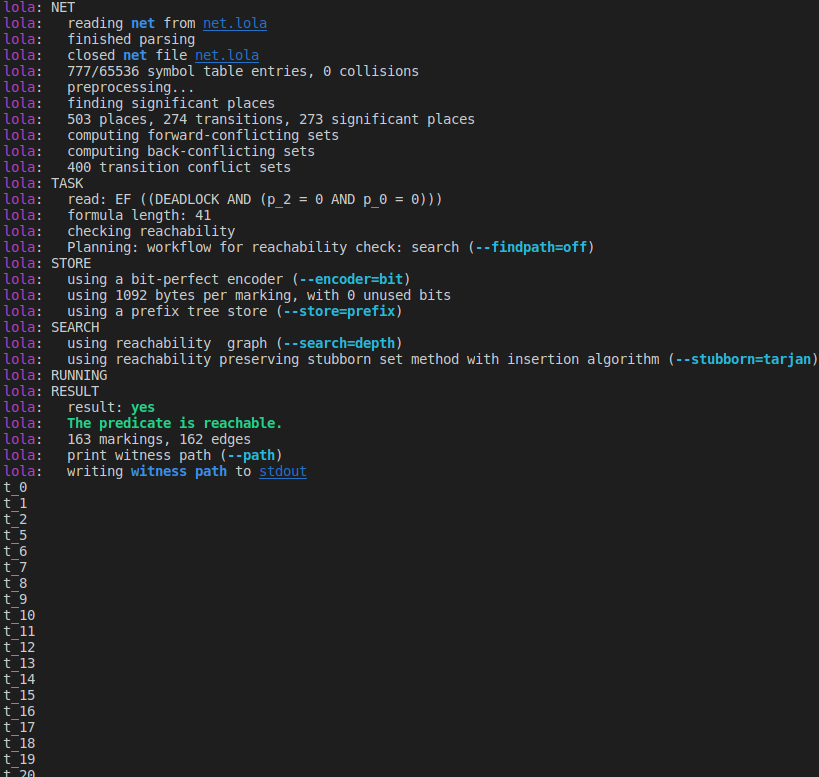
\includegraphics[width=1\textwidth]{./pictures/lola_output.png}
  \caption{LoLA output}
  \label{lola_output}
\end{figure}
Of course we want to use our translation further for verification.
Using our formula on the deadlock program from listing \ref{deadlock_program}, LoLA does find a deadlock and can produce a witness path as shown in figure \ref{lola_output}.
In contrast, if we remove the last line of the program, no deadlock is detected.
Following the witness path in the deadlock case, does indeed lead to the transitions that are involved in the mutex emulation (the mutex place is empty causing involved transitions to be dead).
Earlier tests have also shown that the mutex emulation discussed in chapter \ref{emulation} is necessary to produce deadlocks.
Without the information on where and how execution should be blocked, the translation process cannot infer this behavior.
This is a general problem for blocking behavior by external cause.

At this point it might be adequate to add that active waiting (looping until a guard has an expected value) is not a deadlock and also would not be detected with this approach.
However, it is likely that another formula can be found, to verify that leaving the waiting section is always possible.
But again this most likely would require to consider the values that variables can hold and therefore high-level semantics.

\chapter{Evaluation}
\label{eval}
The results show that our basic approach can be used to verify some basic properties.
And even though the state of the translation is nowhere near productive use there are some lessons learned that we can discuss.
\section{The Model}
The main draw back that followed us for the entire process is the abstraction of data in low-level Petri-Nets.
Advantages of the low-level model are not only the reduced complexity and higher verification performance, it can also produce stricter assertions.
Additionally, our particular model most likely can exploit a Petri-Net property called safety:
if we overlook the workaround for compensating the missing storage-statements, the token count on every place cannot exceed a maximum of one.
One obvious use for that property is the state encoding for every place, which can be done with a single bit this way.
This might be helpful for very large programs with lots of places.

The greatest disadvantage of low level Petri-Nets is the reduced expressiveness of data.
While flow related properties are easy to model with simple tokens, as soon as we enter the realm of data related properties, we have to make compromises.
The approach we took models every interaction with data, but we cannot facilitate their set of possible values for verification tasks.
Another problem is that no moving data is modeled.
If a previously initialized local moves into another local (like a field of a struct), we completely loose this information in our translation.
Although, we can probably exploit Rusts strict borrow checking and aliasing rules to model a much closer relation between data,
both locals are generated independently with their own places and life cycle.
An improvement for a move of a value from one local to another (which is encoded in MIR with a keyword), could be to connect the places with a transition right away.

Another disadvantage of our current model is function inlining.
If a program calls the same function at different places, a separate instance will be inserted at every call site.
This not only makes the net larger, it catches the translation process in an endless loop in recursive functions.

A solution for most of these problems might be high-level Petri-Nets where we can model data verbosely.
With them we could properly model data and detach function calls from the call site.
Only the cost for verification performance remains unknown at the moment.
Some problems, on the other hand, cannot be solved this way.
For example, program parts that are not represented by MIR (like foreign functions and compiler intrinsics) cannot be translated and have to be emulated.
Also, information on blocking behavior is needed to model deadlocks appropriately.
For mutexes we again worked around this issue with emulation.
Additional blocking functionality (like waiting threads) have to be emulated separately.

\section{Verification}
The ability to discover deadlocks is already a useful property for model checking.
But our model is not restricted to this single property.
An easy addition is to check if the panic state is reachable.
Unfortunately virtually every program with a realistic size can panic.
So this property is of limited use unless variable data can be respected.
However, more complex properties could deal with conditional reachability.
For example if a function can be reached from a particular program state.
Or if every execution of a program eventually visits a function or statement.
But then again, our statements would be much stronger if we could consider data values.
